
\section{How To create a simulation}
To create your own simulation, from a xml description, or a c++ file, you have to respect some rules.
The Modeler can be used to have a quick view of all the components already available in Sofa.
\subsection{Model a dynamic object}
To model a dynamic object, you have to follow that steps:
\subsubsection{Mechanical}
\begin{enumerate}
 \item { \bf GNode}: Generally, we give it the name of the whole object
 \item { \bf Solver}: choose the solver you want to resolve this part of the simulation (you might need two components actually, a OdeSolver followed by a LinearSolver)
 \item { \bf Topology}: describes how the dofs will be connected
 \item { \bf MechanicalState}: the degrees of freedom (dofs) of your object. It is the heart of the simulation
 \item { \bf Mass}: the mass attached to each dofs of the object
 \item { \bf ForceField}: describes the behavior of your object, how it will interact. If you don't specify one, your model won't be deformable
 \item { \bf Constraint}: optional
\end{enumerate}

\begin{figure}
	\centering
		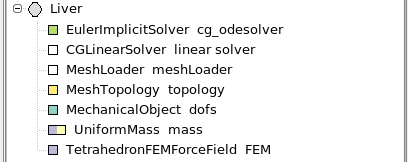
\includegraphics[width=0.5\textwidth]{Modelling0.jpg}
	\caption{Basic example modelling a Finite Element Object}
\end{figure}
After these steps, you will have a mechanical model, that can be integrated in a Sofa Simulation. Nevertheless, you won't have any visual model, only points representing your dofs.


\subsubsection{Visual}
Using the previously described mechanism of Mapping, you can attach a visual model, of any kind, to represent your mechanical object.

\begin{enumerate}
 \item { \bf GNode}: add a GNode inside your current object. It will contain the components necessary to do the visual mapping
 \item { \bf VisualModel}: this component contains the mesh representing your object
 \item { \bf Mapping}: a non-mechanical mapping will connect your mesh to the dofs. This mapping won't transmit forces from your visual model to the dofs. If you are writing...
\begin{itemize}
 \item { \bf a c++ file}, take good care of using a non-mechanical template: The second object should be a template of ExtVec3Types
 \item { \bf a xml file}, you have to specify the path to the two models to be mapped: 
\begin{itemize}
 \item object1=''../..`` : meaning the dofs are located one level below
 \item object2=''Visual`` : where ''Visual'' is the name of your VisualModel (as described in this example, it is located at the same level as your mapping)
\end{itemize}
\end{itemize}
 
\end{enumerate}

\begin{figure}[htpb]
	\centering
		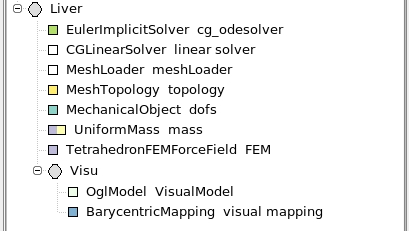
\includegraphics[width=0.5\textwidth]{Modelling1.jpg}
	\caption{Basic example modelling a Finite Element Object with a Visual Model}
\end{figure}
\subsubsection{Collision}
If you need to simulate interactions between objects, you will need another node, a Collision Node.
In the example we describe, we will use a Triangle Model as collision model. We chose it because, it behaves like most of our collision models, needing a topology and dofs to behave properly. But if you use the simple SphereCollisionModel, this component already contains a topology, dofs and collision model. So you will just have to create a mechanical mapping.
\begin{enumerate}
 \item { \bf GNode}: add a GNode inside your current object. It will contain the components necessary to do the mechanical mapping
 \item { \bf Topology}
 \item { \bf MechanicalState}: the dofs of your collision model. They will be used to transmit the forces they receive from the interactions to the real mechanical dofs of your object
 \item { \bf CollisionModel}: the model of collision, a sequence of them can be specified (for example, TriangleModel, then LineModel, then PointModel).
 \item { \bf MechanicalMapping}: for a XML description of your object, you don't need to specify who is object1 or object2
\end{enumerate}

\begin{figure}[htpb]
	\centering
		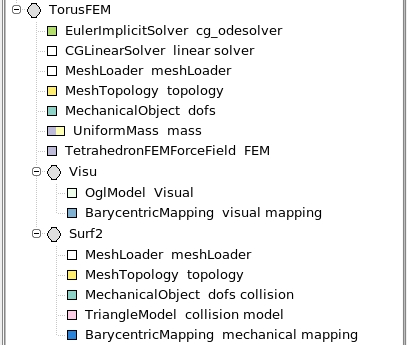
\includegraphics[width=0.5\textwidth]{Modelling2.jpg}
	\caption{Basic example modelling a Finite Element Object with a Visual Model and CollisionModel}
\end{figure}

Your object is now ready to be inserted in a Sofa simulation.

Another example of a full object, using SphereModels.
\begin{figure}[htpb]
	\centering
		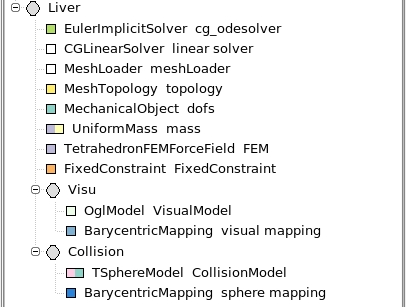
\includegraphics[width=0.5\textwidth]{Modelling3.jpg}
	\caption{Modeling a liver with sphere collision model}
\end{figure}

\subsection{Model a static object}
Fixed object, like floors, walls, or objects that only must be used as obstacle are easier to model. 

\begin{enumerate}
 \item { \bf GNode}: Generally, we give it the name of the whole object
 \item { \bf Topology}: describes how the dofs will be connected
 \item { \bf MechanicalState}: the degrees of freedom (dofs) of your object
 \item { \bf CollisionModel}: the model of collision, a sequence of them can be specified (for example, TriangleModel, then LineModel, then PointModel). You have to specify the fact that your object is fixed by setting some flags.
\begin{itemize}
 \item { \bf moving}: if your object can be displaced. You can think of an external interaction, using an haptic device for instance
 \item { \bf simulated}: if you object is controlled by a simulation. Generally, a fixed object is not simulated.
\end{itemize}
 \item { \bf VisualModel}: this component contains the mesh representing your object
\end{enumerate}
No need of any mapping as no forces, or modifications of position will be transmitted.

\begin{figure}[htpb]
	\centering
		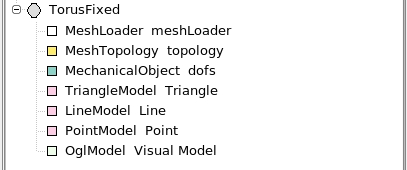
\includegraphics[width=0.5\textwidth]{Modelling4.jpg}
	\caption{Modeling a Fixed object}
\end{figure}


\subsection{Include Collisions}
To perform collision detection, as you have seen, the objects of the scene must have a or several collision models. But, you will have to set up several components performing the collision detection, and response.

\begin{enumerate}
 \item { \bf CollisionPipeline}: currently, only our default collision pipeline is available.
 \item { \bf CollisionDetection}: method to detect collisions
 \item { \bf IntesectionMethods}: depending on the collision detection algorithm, you may have to specify some components to perform the proximity intersection test for example.
 \item { \bf ContactManager}: receiving the collisions found, it will generate a response. You can chose the response you want by filling the field ``response''. By default, we use a penalty response.
 \item { \bf CollisionGroupManager}: manages collisions between different kind of simulated objects. It avoids explosions of your simulation by changing the graph dynamically, and putting an appropriated solver above the objects in interaction
\end{enumerate}

\begin{figure}[htpb]
	\centering
		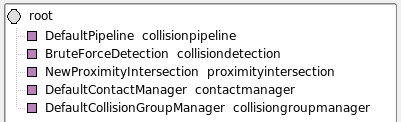
\includegraphics[width=0.5\textwidth]{Modelling5.jpg}
	\caption{Collision Components}
\end{figure}
